\chapter{Feasibility Study of a Pixelated \lartpc{} for the \dune{} Near Detector}
\label{chap:dune-nd}

\todo[inline]{More details on statistics?}

With \AC{} selected as  the \lar{} component of the \dune{} near detector (ND), there were two main question that needed to be addressed:
\begin{enumerate}
	\item Is a pixelated \lartpc{} feasible?
	\item Can the \lar{} detector handle the high rates?
\end{enumerate}
Number one is addressed in Chapter~\ref{chap:viper}.
This chapter will address question number two.


\section{The Argon Box Simulation Tool}
\label{sec:dune-nd_argon-box}

Argon Box\footnote{\url{https://github.com/dadwyer/argon_box}} was developed with the goal of providing an easy-to-use simulation of particle interactions in \lar{} component of the ND.
At the time of this writing its feature set is quite limited, in particular it does not incorporate any other detector materials except for the box of argon.
Primary particles can either be provided by a particle gun (e.g.\ \Pem, \Pn, \Pp, \Pgmp) or in form of a \emph{HEPEVT} file---a file format standard for passage of particle events between different simulation tools.
For this study, several million neutrino events were produced with the GENIE\footnote{\url{https://genie.hepforge.org}} neutrino event generator.
Secondary particle transport and interaction in Argon Box is performed by Geant4.\footnote{\url{http://geant4.cern.ch}}
Finally, the energy deposition in \lar{} is voxelised and stored together with all the necessary ancillary information about the depositing particle.
The data is stored in the tree format of the ROOT data analysis framework.\footnote{\url{https://root.cern}}
This allows for convenient further processing using ROOT.


\section{\Pgpz pile-up study}
\label{sec:dune-nd_pile-up}

A significant amount of \Pgpz are produced in several resonant and coherent neutrino interactions (see Table~\ref{tab:nu-detection_nd-rates} Section~\ref{sec:nu-detection_interactions} and~\cite{dune2}).
They decay according to
\begin{IEEEeqnarray}{C}
	\HepProcess{\Pgpz \to \Pgg\Pgg}
\end{IEEEeqnarray}
with a branching ratio of \SI{98.8}{\percent}\cite{pdg}.
The photons subsequently produce electromagnetic showers in \lar{} (see Section~\ref{sec:nu-detection_fs}).
At the energies of the \dune{} beam (see Figure~\ref{fig:nu-detection_dune-flux}), most showers do not deposit a homogenous cone of charge but rather a lot of individually resolvable \Pepm tracks.
More importantly, there often are significatn gaps in betweend these charge clusters.
A main challenge of shower reconstruction is to associate these well separated charge blobs to the correct event.
Misidentiions lead to a misreconstruction of the neutrino energy.
The resulting discrepancy to the true neutrino energy has the potential to skew the measured energy spectrum and, thus, influence the oscillation measurements.
The complexity of reconstruction paired with the potential impact on the physics measurements makes photons produced by \Pgpz decays a good sample to study the robustness to pile-up of a pixelated \lartpc{} in the \dune{} ND environment.

\begin{table}[htb]
	\centering
	\caption{Parameters of the \Pgpz pile-up simulation.}
	\label{tab:dune-nd_pile-up-params}
	\begin{tabu} to \textwidth {|l|S|}
		\hline
		{Beam direction} &			{$Z$ (positive)} \\
		\hline
		{Gravitation} &				{$Y$ (negative)} \\
		\hline
		{Resolution $X$} &			\SI{3}{\milli\metre} \\
		\hline
		{Resolution $Y$} &			\SI{3}{\milli\metre} \\
		\hline
		{Resolution $Z$} &			\SI{3}{\milli\metre} \\
		\hline
		{Target volume $X$} &		\SIrange{-1000}{5000}{\milli\metre} \\
		\hline
		{Active volume $X$} &		\SIrange{0}{4000}{\milli\metre} \\
		\hline
		{Fiducial volume $X$} &		\SIrange{300}{3700}{\milli\metre} \\
		\hline
		{Target volume $Y$} &		\SIrange{-1000}{3500}{\milli\metre} \\
		\hline
		{Active volume $Y$} &		\SIrange{0}{2500}{\milli\metre} \\
		\hline
		{Fiducial volume $Y$} &		\SIrange{300}{2200}{\milli\metre} \\
		\hline
		{Target volume $Z$} &		\SIrange{-4000}{5000}{\milli\metre} \\
		\hline
		{Active volume $Z$} &		\SIrange{0}{5000}{\milli\metre} \\
		\hline
		{Fiducial volume $Z$} &		\SIrange{300}{4700}{\milli\metre} \\
		\hline
		{Detection threshold} &		\SI{0.1}{\mega\electronvolt} \\
		\hline
		{Cone extent} &				{$10 X_{\m{0}} = \SI{1400}{\milli\metre}$} \\
		\hline
		{Cone half opening angle} &	\ang{15} \\
		\hline
		{Cylinder radius} &			\SI{25}{\milli\metre} \\
		\hline
		{Beam intensity} &			{$\SI{2}{\mega\watt} \widehat{=} \SI{0.2}{evt\per\tonne}$} \\
		\hline
	\end{tabu}
\end{table}

To investigate the effects of pile-up on energy reconstruction, a working reconstruction algorithm is necessary.
However, at the time of writing, official reconstruction tools were only available for \lartpc{}s read out by wire planes.\footnote{\url{http://larsoft.org}}
Therefore, a rather primitive algorithm for true 3D space points was implemented, under the assumption that a positive outcome of such a pile-up study would imply an even better performance of a more sophisticated reconstruction.
This algorithm is explained in the following.
All its parameters are listed in Table~\ref{tab:dune-nd_pile-up-params}.

\begin{figure}[htb]
	\centering
	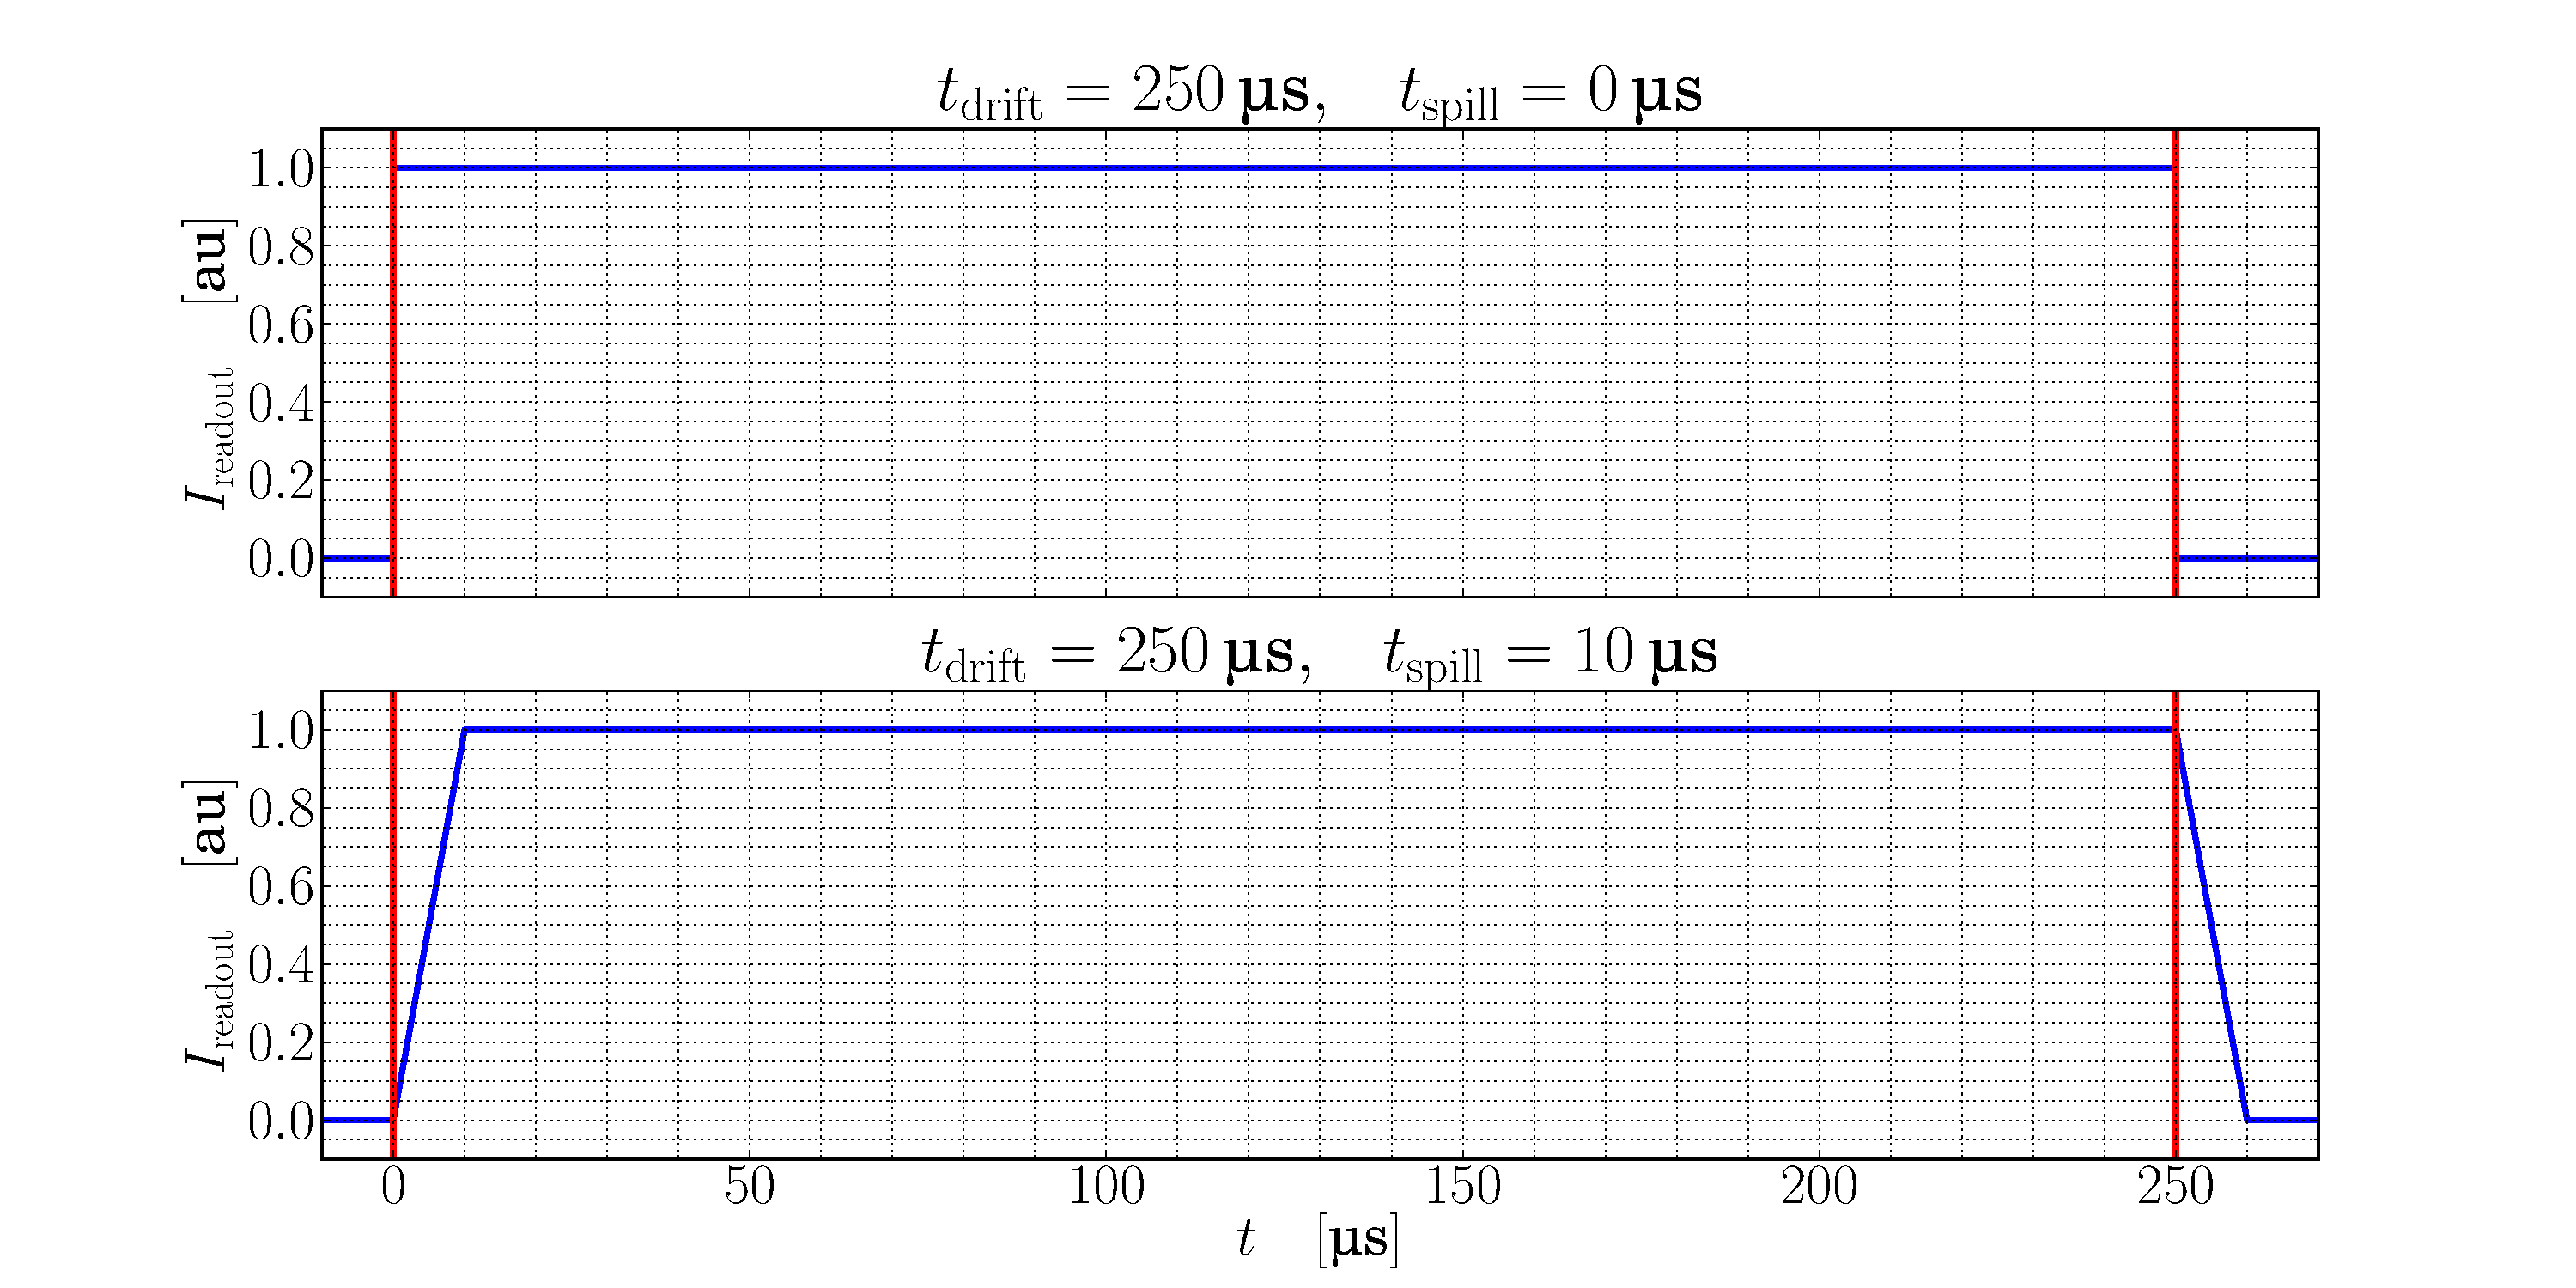
\includegraphics[width=\textwidth]{pile-up/charge_flux}
	\caption{Average current collected by the readout for one spill as a function of time.
	The current is given in arbitrary but equal units for both plots.
	The upper plot assumes the whole charge is deposited instantaneously while for the lower plot, the actual spill duration from~\cite{dune2} is used.}
	\label{fig:dune-nd_charge-flux}
\end{figure}

The basic underlying assumption is that a non-multiplexed pixel readout will yield unambiguous 3D space points of charge deposition with a given resolution, depending on the geometry of the pixel plane, time resolution of the readout electronics, and charge transport effects.
Furthermore, it is assumed that EM shower can be identified and their starting point and direction reconstructed with negligible errors and inefficiencies, i.e.\ this information is taken from the simulation truth.
A cone is calculated in the direction of the shower with its tip at the first charge deposition of the initial photon.
The opening angle and longituginal extent of the cone were optimised by looking at the distributions of the distance from the starting point and angle w.r.t. the direction of the shower.
The finite resolution of the detector is emulated by voxelising the charge deposition with the corresponding resolution in all three spatial coordinates.
This leads to problems near the tip of the cone where the transversal extent is lower than the voxel dimensions.
In particular, it can happen that most of the initial charge is shifted outside the cone.
Furthermore, multiple scattering at lower energies makes the cone model suboptimal near the tip.
Therefore, the acceptance volume for the reconstruction is taken as the union of the cone with a cylinder around the direction of the shower of the same longitudinal extent as the cone.

\begin{figure}[htb]
	\centering
	\includegraphics[width=\textwidth]{pile-up/2MW/eff_pur}
	\caption{Efficiency (accepted true over total true energy deposition) and purity (accepted true over total accepted energy deposition) distributions of a simple cone-cylinder union EM shower reconstruction algorithm.
	The distribution represents the fraction of photons produced by \Pgpz whose energy was reconstructed with the corresponding efficiency/purity.
	Purity is shown for four different selections of misidentified energy: total (magenta); deposited by other events only (cyan); deposited by other events only, excluding muons (red), deposited by photons and neutrons from other events only (blue).
	The simulated beam intensity is \SI{2}{\mega\watt}.}
	\label{fig:dune-nd_2MW-eff-pur}
\end{figure}

Argon Box propagates the neutrino interaction events it gets from GENIE through liquid argon, the output is a ROOT tree of neutrino interaction events.
To get a realisitc simulation of beam events in the detector, these events need to be distributed randomly in time and space.
Beam spills are simulated by drawing the number of events for each spill from a Poisson distrubition whose mean is calculated from the beam intensity and the target mass.
The resulting number of events is taken from the Argon Box ROOT tree and their vertices are placed within the \lar{} volume at coordinates drawn from a uniform distribution.

\begin{figure}[htb]
	\centering
	\includegraphics[width=\textwidth]{pile-up/2MW/energy_error}
	\caption{Fractional error on the reconstructed neutrino energy due to missed or misidentified energy depositions as a function of true neutrino energy.
	Misidentified energy is shown for three different selections: total deposited by other events (cyan); deposited by other events excluding muons (red), deposited by photons and neutrons from other events only (blue).
	The simulated beam intensity is \SI{2}{\mega\watt}.}
	\label{fig:dune-nd_2MW-energy-error}
\end{figure}

Three different argon volumes are assumed for the simulation: target, active, and fiducial volume.
The actual detector dimensions are represented by the active volume.
It is inside the target volume which is the volume within which the neutrino vertices are placed randomly.
This is done as a crude emulation of rock events, secondary particles from beam neutrino interactions outside the detector volume.
The additional target mass is \SI{1}{\metre} in all four directions transverse to the beam, and \SI{4}{\metre} in upstream beam direction.
Finally, a fiducial volume \SI{0.3}{\metre} ($\approx 2 X_{\m{0}}$) smaller than the active volume on all six faces is defined.
Without the latter, there is a significant number of photons produced by \Pgpz decays inside the detector but only showering outside the detector.
Table~\ref{tab:dune-nd_pile-up-params} contains a summary of all the \lar{} volume dimensions.

\begin{figure}[htb]
	\centering
	\includegraphics[width=\textwidth]{pile-up/2MW_XZ/eff_pur}
	\caption{Efficiency (accepted true over total true energy deposition) and purity (accepted true over total accepted energy deposition) distributions of a simple cone-cylinder union EM shower reconstruction algorithm.
	The distribution represents the fraction of photons produced by \Pgpz whose energy was reconstructed with the corresponding efficiency/purity.
	Purity is shown for four different selections of misidentified energy: total (magenta); deposited by other events only (cyan); deposited by other events only, excluding muons (red), deposited by photons and neutrons from other events only (blue).
	The simulated beam intensity is \SI{2}{\mega\watt}.
	As a primitive simulation of a wire readout, only X and Z coordinates are used for the energy reconstruction.}
	\label{fig:dune-nd_2MW-XZ-eff-pur}
\end{figure}

Another issue of concern is the influence of drift time.
This is the actual cause of event pile-up; if the detector was infinitely fast, all neutrino interactions could be separated in time.
In reality, even the \AC{} TPCs with a drift length of only \SI{0.5}{\metre}, corresponding to a full readout cycle of \SI{250}{\micro\second}, are significantly slower than the spill duration of \SI{10}{\micro\second} of the \dune{} beamline reference design.~\cite{dune2}
Figure~\ref{fig:dune-nd_charge-flux} visualises this effect.
The charge arriving at the readout is represented as an average current in arbitrary units (the same for top and bottom, though).
The magnitude of this readout current is a direct measure for event pile-up in the corresponding time slice.
For simplicity, an infinitely short spill duration was assumed for the pile-up study (top), i.e.\ the whole ionisation charge produced by one beam spill is deposited instantaneously inside the TPC volume.
As the time in between beam spills is $\order{\SI{1}{\second}}$, all this charge can be read out within one drift time.
In this case, the average current (pile-up) seen by the readout is constant over the whole readout cycle.
The realistic case with the spill duration of the reference beam is depicted in the bottom plot.
At the beginning of the readout cycle, there is no charge deposited yet, the current (pile-up) is zero.
Over the duration of the beam spill, ionisation charge accumulates inside the TPC volume while the exisiting charge is transported towards the readout by the drift field.
After the beam spill is over, the remainder of the initial drift volume (\SI{240}{\micro\second}) contains a uniform charge density.
The additional \SI{10}{\micro\second}, in front of the cathode and part of the next readout cycle, again, contain a ramped charge density with zero charge at the cathode, corresponding to the end of the spill.
In short, a spill duration shorter than but comparable to the drift time results in the shape of the ionisation current (event pile-up) seen over time to become a trapecoid rather than a square.
The integral, i.e.\ the total ionisation charge (deposited energy) is the same but part of it is shifted from the spill time slice to the beginning of the next readout cycle.
Similarly, the peak current (pile-up) is the same, as long as the spill duration is shorter than the drift time.
If the spill duration becomes longer than the drift time, the charge is distributed over more then two readout cycles and the peak current (pile-up) begins to decrease.
Therefore, the assumption of an infinitely short spill is a worst-case scenario slightly improved by the real, finite spill duration.
However, for most of the drift time (\SI{240}{\micro\second}), pile-up is the same.

\begin{figure}[htb]
	\centering
	\includegraphics[width=\textwidth]{pile-up/2MW_XZ/energy_error}
	\caption{Fractional error on the reconstructed neutrino energy due to missed or misidentified energy depositions as a function of true neutrino energy.
	Misidentified energy is shown for three different selections: total deposited by other events (cyan); deposited by other events excluding muons (red), deposited by photons and neutrons from other events only (blue).
	The simulated beam intensity is \SI{2}{\mega\watt}.
	As a primitive simulation of a wire readout, only X and Z coordinates are used for the energy reconstruction.}
	\label{fig:dune-nd_2MW-XZ-energy-error}
\end{figure}

After all events of one spill are placed inside the target volume, all \Pgpz photons produced inside the fiducial volume are reconstructed using the cone algorithm.
All energy depositions inside the active volume are considered.
To assess the performance of the performance of the algorithm, the following quantities are computed for each photon:
\begin{description}
	\item[Efficiency] is the ratio of correctly accepted energy deposition inside the cone-cylinder union to total true energy deposition of the photon.
		This is a measure for the performance of the reconstruction and can be used to ensure optimum tuning of the union parameters.
	\item[Purity] is the ratio of correctly accepted energy deposition inside the cone-cylinder union to total accepted energy deposition inside the union.
		This is a measure for event pile-up.
		The higher the amount of charge deposition from other events inside the union, the lower the purity.
\end{description}
Using this general definition of purity leads to quite mediocre results.
However, there are some assumptions that can be taken even without knowing the actual reconstruction algorithm.
The incorrectly accepted energy deposition inside the cone-cylinder union can be limited to energy deposited by other events; misidentified energy from the same event does not affect the total reconstructed neutrino energy.
From results of earlier experiments\todo{sauce}, the muon reconstruction can be assumed to be very efficient.
Assuming \SI{100}{\percent} reconstruction efficiency for muons and \SI{0}{\percent} for all other particles can therefore serve as a lower limit for the purity.
It can be calculated by ignoring misidentified muon energy depositions.
On the other hand, an upper limit for the purity can be calculated by assuming \SI{100}{\percent} reconstruction efficiency for all charged particles and \SI{0}{\percent} for neutral particles (\Pgpz and \Pgg).
This is calculated by only taking into account misidentified energy deposited by neutral particles.
Assuming \SI{0}{\percent} reconstruction efficieny for neutral particles might lead to a slight underestimation of purity.
However, this effect should be more than compensated by the overestimation of the charged particle reconstruction efficiency, given the highly complex nature of reconstructing unconnected clusters from neutral particles.
Therefore, this upper purity limit should hold at least in the near future.

\begin{figure}[htb]
	\centering
	\includegraphics[width=\textwidth]{pile-up/10MW/eff_pur}
	\caption{Efficiency (accepted true over total true energy deposition) and purity (accepted true over total accepted energy deposition) distributions of a simple cone-cylinder union EM shower reconstruction algorithm.
	The distribution represents the fraction of photons produced by \Pgpz whose energy was reconstructed with the corresponding efficiency/purity.
	Purity is shown for four different selections of misidentified energy: total (magenta); deposited by other events only (cyan); deposited by other events only, excluding muons (red), deposited by photons and neutrons from other events only (blue).
	The simulated beam intensity is \SI{10}{\mega\watt}.}
	\label{fig:dune-nd_10MW-eff-pur}
\end{figure}

The results of the pile-up study are shown in Figures~\ref{fig:dune-nd_2MW-eff-pur} through~\ref{fig:dune-nd_10MW-energy-error}.
Figures~\ref{fig:dune-nd_2MW-eff-pur} and~\ref{fig:dune-nd_2MW-energy-error} assume optimised beam intensity of \SI{2}{\mega\watt}.
Efficiency and purity distributions are plotted in Figure~\ref{fig:dune-nd_2MW-eff-pur} as the fraction of \Pgpz photons reconstructed with the respective efficiency/purity.
It can be seen, that purity significantly improves under the assumptions described above.
In particular, taking the mentioned lower and upper limits for pile-up, \SIrange{50}{60}{\percent} of the photons experience no pile-up at all.
While these distributions give a general idea of pile-up, there usefulness for an assessment from a physics point of view is limited.
Therefore, the actual impact on the reconstructed neutrino energy as a function of the true neutrino energy was calculated and plotted in Figure~\ref{fig:dune-nd_2MW-energy-error}.
The y-axis represents the fractional error on the reconstructed neutrino energy and the colors correspond to the same selections as for the purity/efficiency plot in Figure~\ref{fig:dune-nd_2MW-eff-pur}.
However, only misidentified energy from other events affects the total reconstructed energy of the neutrino which is why the magenta selection, including misidentified energy from the same event, is not applicable to this calculation.
It can be seen, that the effect of missed energy starts at a few~\si{\percent} for the lower neutrino energies and the quickly goes down to stabilise around \SI{1}{\percent}.
This indicates that the cone-cylinder union algorithm, eventhough quite primitive, performs reasonably well.
The error due to misidentified energy starts at around \SI{10}{\percent} and then, settles between \SIrange{1}{2}{\percent}.

\begin{figure}[htb]
	\centering
	\includegraphics[width=\textwidth]{pile-up/10MW/energy_error}
	\caption{Fractional error on the reconstructed neutrino energy due to missed or misidentified energy depositions as a function of true neutrino energy.
	Misidentified energy is shown for three different selections: total deposited by other events (cyan); deposited by other events excluding muons (red), deposited by photons and neutrons from other events only (blue).
	The simulated beam intensity is \SI{10}{\mega\watt}.}
	\label{fig:dune-nd_10MW-energy-error}
\end{figure}

To get a rough idea of the performance of a 2D wire readout in the same environment, the same study was performed ingoring the Y coordinate completely, leaving everything else untouched.
Of course, this is a gross underestimation of the capabilities of existing reconstruction algorithms for 2D charge readout data.
In particular, contemporary experiments use at least three 2D projections whereas only one was used here.
Eventhough, doing this comparison serves to show that the simple cone-cylinder union reconstruction algorithm breaks down for two dimensions as can be seen in Figures~\ref{fig:dune-nd_2MW-XZ-eff-pur} and~\ref{fig:dune-nd_2MW-XZ-energy-error}.
The fraction of events not suffering from pile-up is below \SI{10}{\percent} while the error on energy reconstruction has increased to \SIrange{5}{10}{\percent} at high energies and event \SIrange{20}{40}{\percent} at low energies.
Efficiency and energy error due to missed energy are comparable eventhough, the cone and cylinder dimensions are no longer correct for photons not parallel to the XZ plane.

Finally, as a cross-check, the (3D) pile-up study was performed for a hypotheticel \SI{10}{\mega\watt} beam.
As expected, pile-up increases drastically while efficiency does not change much as can be seen in Figures~\ref{fig:dune-nd_10MW-eff-pur} and~\ref{fig:dune-nd_10MW-energy-error}.

In summary, this study shows that even a very primitive EM shower reconstruction algorithm, employing a cone-cylinder union selection, performs well in the high-multiplicity environment of the \dune{} ND, when fed with unambiguous 3D spatial coordinates of energy depositions.
It clearly fails when reduced to two dimensions or presented with a much higher beam intensity.